\subsection{\ref{exp:design:1} - HTTP Maximum Throughput}
\label{sec:experiments:results:per-experiment:01}
% Goal:
% To find the maximum throughput each of the meshed configurations can achieve.

\begin{figure}
\centering
\makebox[\linewidth][c]{
    \begin{minipage}{.6\textwidth}
      \centering
      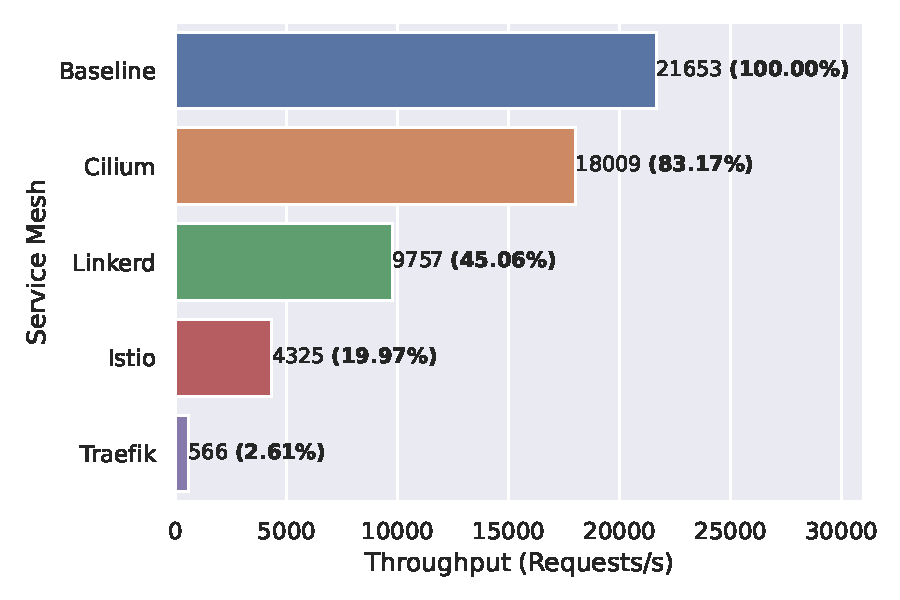
\includegraphics[width=\linewidth]{5_experimental_evaluation/figures/exp-01-max-throughput.pdf}
      \caption[Average throughputs of \gls{sm} systems under maximum load.]{Average throughputs of \gls{sm} systems under maximum load.}
      \label{fig:exp:01:maximum-throughput}
    \end{minipage}
    
    
    \begin{minipage}{.6\textwidth}
      \centering
      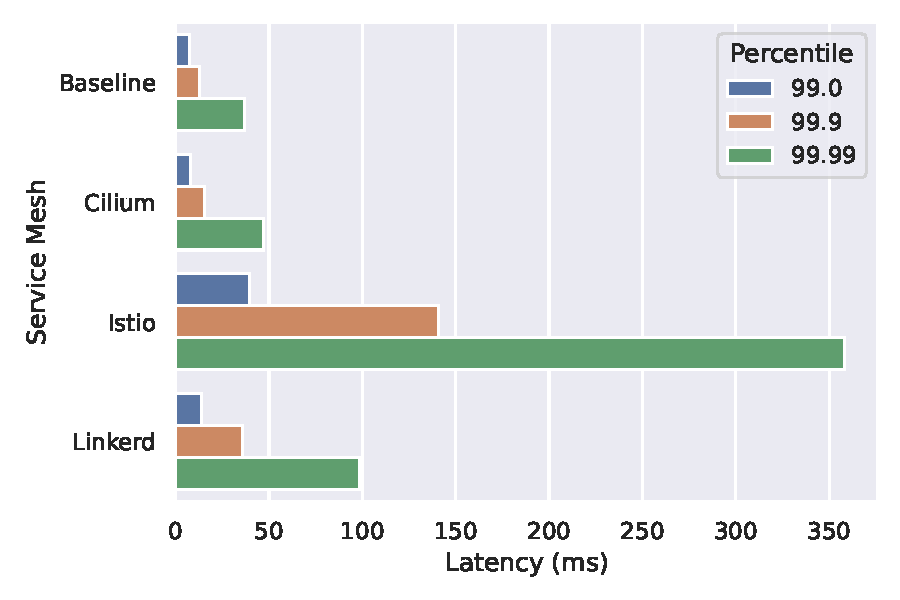
\includegraphics[width=\linewidth]{5_experimental_evaluation/figures/exp-01-tail-latencies.pdf}
      \caption[Tail end latencies of \gls{sm} systems under maximum load.]{Tail end latencies of \gls{sm} systems under maximum load.}
      \label{fig:exp:01:tail-end-latencies}
    \end{minipage}
}
\end{figure}



The first experiment evaluates the \gls{sm} systems when they are fully satiated, i.e. they are at full capacity and handling the maximum amount of load that they can process. This amount of load, or throughput, is expressed in the number of requests per second the system can process.

\subsubsection{Maximum Sustained Throughput Analysis}
\label{sec:experiments:results:per-experiment:01:throughput}

In \cref{fig:exp:01:maximum-throughput} we present a bar chart which depicts the average throughput a \gls{sm} system was able to process throughout the duration of the experiment. On the y-axis we present the different \gls{sm} configurations, whereas the x-axis represents the throughput in requests per second. Next to each bar we present the actual observed value and the percentage of throughput a system was able to process compared to the  best performing configuration, which in this case is the baseline.

From these results, we can derive that all the \gls{sm} systems experience a loss of throughput compared to the baseline configuration. We can relate this observation to the fact that the \gls{sm} systems introduce additional components in the form of proxies in the critical data path of requests. Every request has to be processed by these proxies, which in turn leads to the decrease in maximum sustained throughput. However, even through the decrease in throughput is expected, the amount of this decrease is rather significant. Cilium is the best performing \gls{sm} configuration in this experiment in terms of throughput. However, it still experienced a massive $16.83\%$ reduction compared to the baseline configuration. This observation leads to our first main finding: 

\begin{shaded*}
    \noindent
    \ref{exp:mf1}: 
    Using a \gls{sm} can lead to a significant decrease in sustained throughput.
\end{shaded*}

Another observation we can make from these results is the amount of variance there is among the evaluated \gls{sm} systems. We already established that Cilium is the best performing \gls{sm} system in terms of throughput, even though it had a significant reduction compared to the baseline configuration. This reduction in throughput, however, is little compared to the performance of other configurations. The configuration using Linkerd led to a $54.94\%$ reduction and Istio saw a staggering $80.09\%$ reduction in throughput. The worst performing configuration was using Traefik. This configuration only managed to serve a tiny fraction of the requests and experienced a massive $97.39\%$ reduction in throughput compared to the baseline configuration. From these observations, we can conclude that there is a large variance in the observed throughputs among \gls{sm} systems, where the reductions in throughput range from $16.83\%$ to $97.39\%$. This leads to our second main finding:

\begin{shaded*}
    \noindent
    \ref{exp:mf2}: 
    There is a significant variance in the amount of sustained throughput that \gls{sm} systems can handle.
\end{shaded*}

\subsubsection{Latency Analysis}
\label{sec:experiments:results:per-experiment:01:latency}

In our previous analysis we looked at the amount of requests a configuration can handle. In this part of the analysis we take a look at the durations of the requests themselves. We measure the latency of each request. These latencies represent the time it takes for a request to complete. This is measured from the moment the workload generator sends a request until it successfully receives a response from the target service.

To fully understand the impact that the values and distributions in this analysis can have on real-world application performance, we have to refer to the manner in which applications are often constructed. When using a service-oriented architecture, and namely one using the granularity of microservices, you create an application of many interconnected services. Applications can consist of thousands of microservices \cite{design-example-microservices, netflix-microservices-cost} and a user can indirectly use hundreds of backing services. To evaluate latencies in such a model, we follow the practices as described in the works of Gil Tene \cite{Tene2015-measure-latency}. Because of this model, the tail end latencies are more common than one might expect due to the nature of probabilities. As an example, the ~99.995th percentile of latencies will be experienced in a procedure involving 200 microservices in more than 99\% of the time. 


\begin{figure}
\centering
\makebox[\linewidth][c]{
    \begin{subfigure}{.6\textwidth}
      \centering
      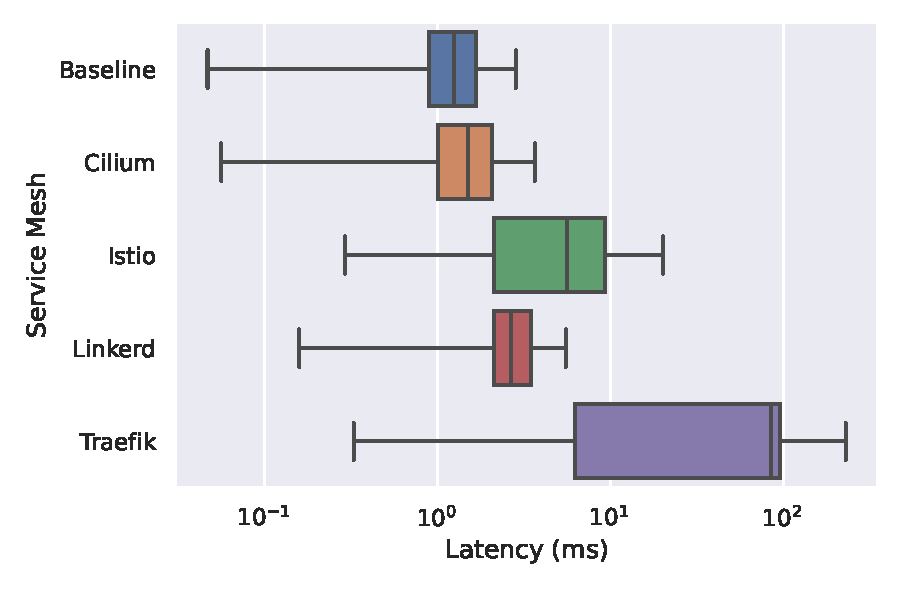
\includegraphics[width=\textwidth]{5_experimental_evaluation/figures/exp-01-latency-log.pdf}
      \caption{Logarithmic scale}
      \label{fig:exp:01:boxplots-latency:log}
    \end{subfigure}
    
    
    \begin{subfigure}{.6\textwidth}
      \centering
      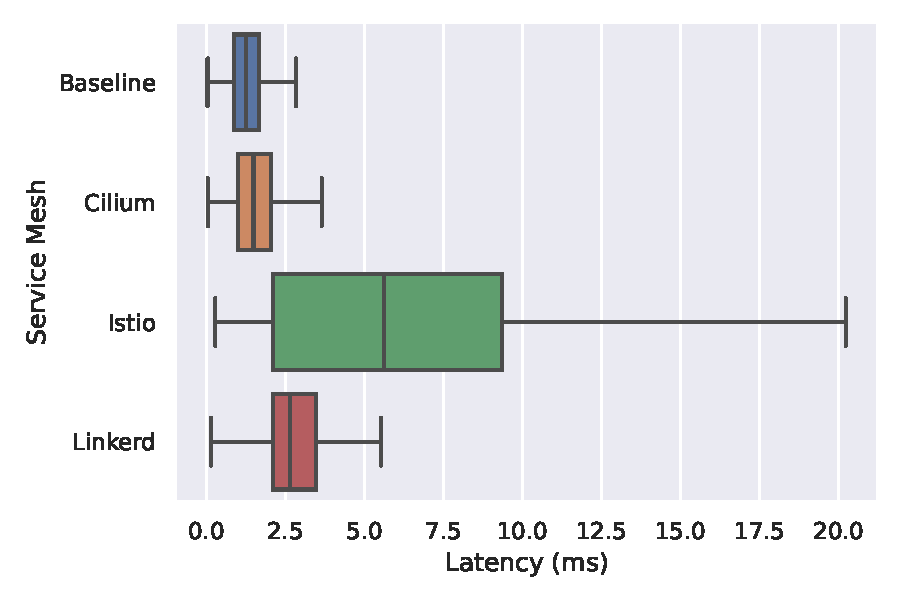
\includegraphics[width=\textwidth]{5_experimental_evaluation/figures/exp-01-latency-no-traefik.pdf}
      \caption{Linear scale, excluding Traefik}
      \label{fig:exp:01:boxplots-latency:linear}
    \end{subfigure}
}
\caption[Latency distributions of \gls{sm} systems under maximum load]{Latency distributions of \gls{sm} systems under maximum load.}
\label{fig:exp:01:boxplots-latency}
\end{figure}


In \cref{fig:exp:01:boxplots-latency} we present a pair of box and whiskers plots that depict the locality, spread and skewness of latencies per \gls{sm} configuration. The lines at the borders of the box represent the 25th and 75h percentiles of data. The line in the middle of the box depicts the median observed value and the whiskers of the box represent the minimum and maximum values. It is important to note that the outliers are omitted from these figures, as we cover these in greater detail later on. The plots depicted in the figure share the meaning of their axes, where the y-axis represents the \gls{sm} configuration and the x-axis represent the observed latencies in milliseconds. The first plot (\cref{fig:exp:01:boxplots-latency:log}), shows all the \gls{sm} configurations and displays the box plots on a logarithmic scale. The second plot (\cref{fig:exp:01:boxplots-latency:linear}), displays the data on a linear scale but excludes Traefik.

In \cref{fig:exp:01:boxplots-latency:log} we present the observed latencies on a logarithmic scale. We do this because it shows that the observed latencies for Traefik surpass the other configurations by an order of magnitude. This leads us to a third main finding:



In \cref{fig:exp:01:boxplots-latency:linear} we compare the \gls{sm} configurations on a linear scale and exclude Traefik. From these results, we can observe that the distribution of observed latencies for Cilium is very similar to that of the baseline configuration. This indicates that the network overhead caused by the in-kernel proxy of Cilium is kept to a minimum which leads us to the third main finding:

\begin{shaded*}
    \noindent
    \ref{exp:mf3}: 
    The network latency overhead caused by the proxy of Cilium is minimal.
\end{shaded*}

Another observation we can make is that Linkerd has a slightly higher median and spread, but is still performing relatively well as it does not deviate too much from the baseline configuration. Istio, on the other hand, appears to suffer significantly more. Not only is the median affected, the spread of observed latencies is significantly greater. We can relate this behaviour to the type of proxy used in their data planes and their design decisions (see \cref{sec:survey:results} \cref{tab:result-proxy}). Whereas Istio uses \textit{Envoy}, a complex and feature rich general purpose proxy, Linkerd uses its own lightweight proxy \cite{linkerd-no-envoy}.


In \cref{fig:exp:01:tail-end-latencies} we present the tail end of latencies observed (above the 99th percentile) for the \gls{sm} configurations excluding Traefik. On the y-axis we represent the latencies observed in millisecond whereas the x-axis represents the various \gls{sm} configurations. The colours of the bars represent a certain percentile of latencies observed.

From the chart in \cref{fig:exp:01:tail-end-latencies} we can observe that Istio suffers the most in the observed tail end latencies. We observed a latency values of 40, 141 and 358 milliseconds for the 99th, 99.9th and 99.99th percentiles respectively. This observation is a continuation from the behaviour depicted in the box and whiskers plot (\cref{fig:exp:01:boxplots-latency:linear}), where the results tied to the configuration using Istio also depicted a large spread in observed latency values. This leads to a fourth main finding:

\begin{shaded*}
    \noindent
    \ref{exp:mf4}: 
    The latencies observed from Istio under load have a large spread, and especially suffer in their tail end.
\end{shaded*}

\begin{figure}
\centering
\makebox[\linewidth][c]{
    \begin{subfigure}{.6\textwidth}
      \centering
      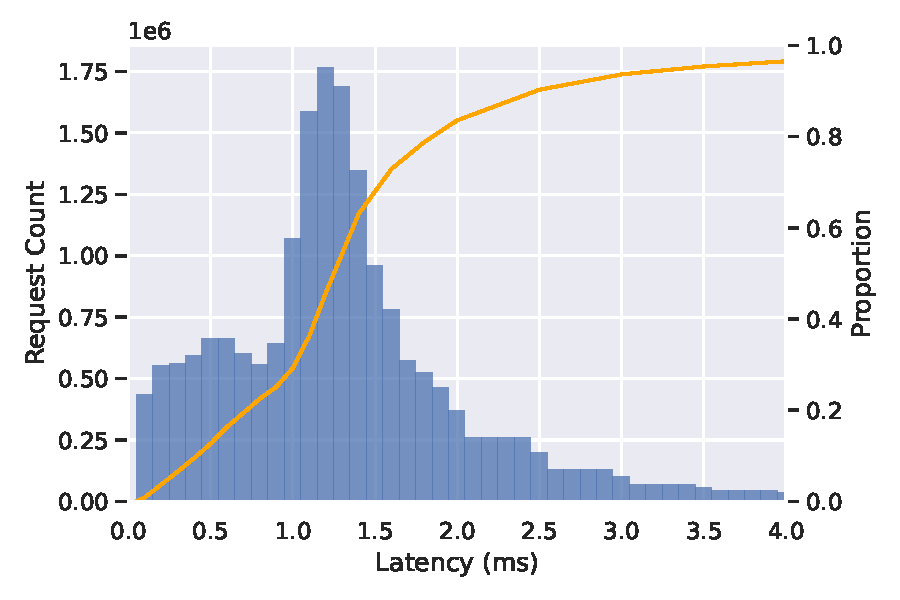
\includegraphics[width=\textwidth]{5_experimental_evaluation/figures/exp-01-latency-distribution-baseline.pdf}
      \caption{Baseline}
      \label{fig:exp:01:histogram:baseline}
    \end{subfigure}
    
    
    \begin{subfigure}{.6\textwidth}
      \centering
      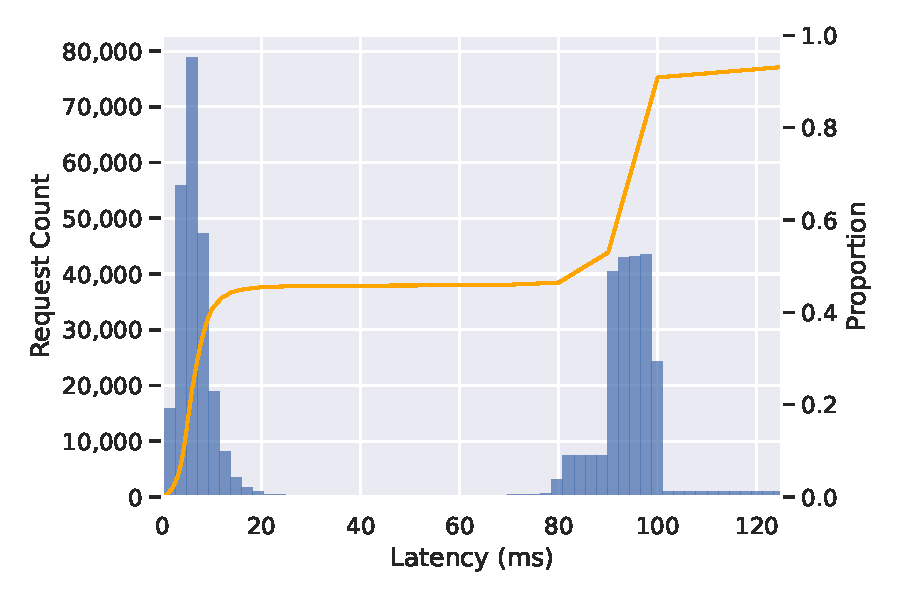
\includegraphics[width=\textwidth]{5_experimental_evaluation/figures/exp-01-latency-distribution-traefik.pdf}
      \caption{Traefik}
      \label{fig:exp:01:histogram:traefik}
    \end{subfigure}
}
\caption[Histogram of observed latencies under maximum load]{Histogram of observed latencies under maximum load per \gls{sm} configuration.}
\label{fig:exp:01:histograms-latency}
\end{figure}

To evaluate the behaviour of Traefik in more detail, we depict the latency distributions in a histogram. In \cref{fig:exp:01:histograms-latency} we depict two plots where each plot contains a histogram of latency distributions. The first plot contains the histogram of the baseline configuration (\cref{{fig:exp:01:histogram:baseline}}) and the second plot contains the histogram of Traefik  (\cref{{fig:exp:01:histogram:traefik}}). Each histogram has a y-axis that represents the number of requests for a specific bin and an x-axis that represents the latency in milliseconds. In addition to the bins, we depict the cumulative density function that shows the proportion of requests smaller than the latency depicted on the x-axis. 

From the results depicted in \cref{fig:exp:01:histograms-latency}, we can observe the distribution of latencies for the baseline configuration and that of Traefik. Note that the values next to the y-axis depict different values, there are more latencies observed for the baseline configuration, as the throughput was not fixed in this experiment. The shape of the distribution for the baseline configuration is similar to that of other configurations except for Traefik (see Appendix for a full comparison). From the shape of the histogram distribution of Traefik we can derive a peculiar finding, it has a bimodal distribution. The first mode is close to 8ms, whereas the second mode is around the 90 milliseconds. These observations lead to our fifth  finding of the experiment: 

\begin{shaded*}
    \noindent
    \ref{exp:mf5}: 
    Traefik mesh performs an order of magnitude worse than any other evaluated service mesh in terms of request latencies when the system is under full load.
\end{shaded*}

\subsubsection{Resource Utilization Analysis}
\label{sec:experiments:results:per-experiment:01:throughput}


\begin{figure}
\centering
\makebox[\linewidth][c]{
    \begin{subfigure}{.6\textwidth}
      \centering
      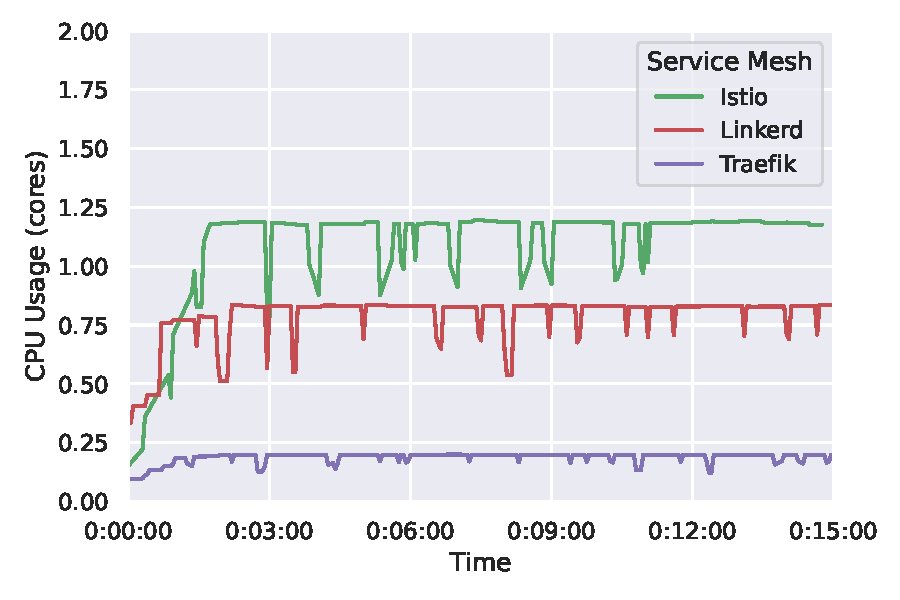
\includegraphics[width=\textwidth]{5_experimental_evaluation/figures/exp-01-cpu-utilization.pdf}
      \caption{CPU Utilization}
      \label{fig:exp:01:resource:cpu}
    \end{subfigure}
    
    
    \begin{subfigure}{.6\textwidth}
      \centering
      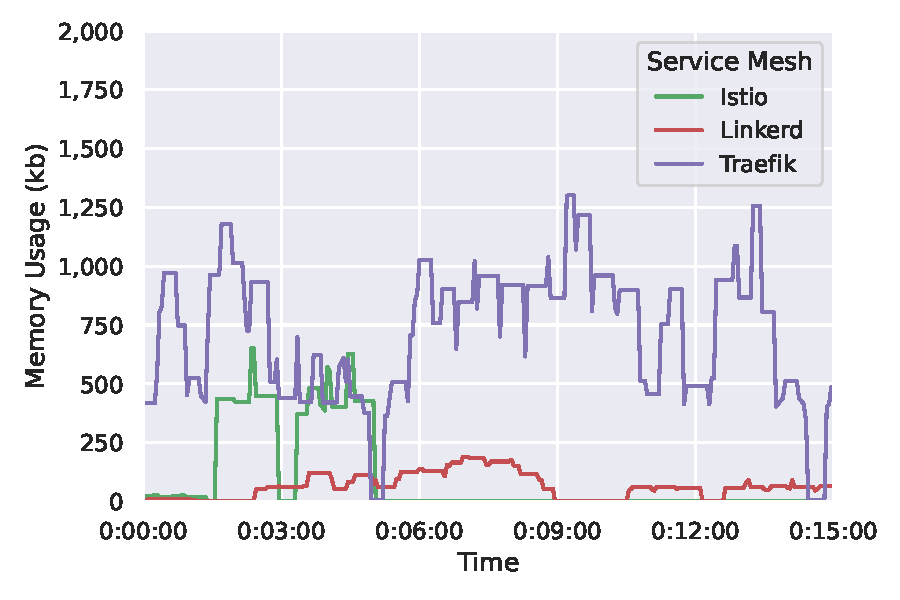
\includegraphics[width=\textwidth]{5_experimental_evaluation/figures/exp-01-memory-utilization.pdf}
      \caption{Memory Utilization}
      \label{fig:exp:01:resource:mem}
    \end{subfigure}
}
\caption[Resource utilization for \gls{sm} systems under load]{Resource utilization for \gls{sm} systems under load}
\label{fig:exp:01:resource-utilization}
\end{figure}


The final type of analysis that we perform is related to the utilization of system resources. In \cref{fig:exp:01:resource-utilization}, we present two line graphs that depict resource usage over time. The first plot (\cref{fig:exp:01:resource:cpu}) is related to the CPU utilization of \gls{sm} proxies. The y-axis represents the fraction of CPU cores used for the \gls{sm} proxy (on a two core system), and the x-axis represents the time delta of the experiment. The second plot depicts \cref{fig:exp:01:resource:mem} the memory utilization. For this, plot the y-axis represents the memory utilization in kilobytes, whereas the x-axis once again represents the time delta of the experiment. In these plots, we display three out of four \gls{sm} systems. This is because we were only able to capture the user-level application containers related to Cilium, and not the kernel-level proxy. For this reason, we omit Cilium from the resource graphs, as the data gathered was inconclusive for that system.

The results as depicted in \cref{fig:exp:01:resource-utilization} show the various configurations under varying levels of load. This means that the comparison cannot be considered fair. With that said, we can still observe some interesting behaviour. In \cref{fig:exp:01:resource:cpu} we depict the CPU utilization for the three observed systems. We can see that the proxy of Istio is the largest consumer of the CPU, even though as previously observed, it had a significantly fewer requests to process compared to Linkerd. This can be related to the aforementioned design decisions of the proxy implementations \cite{linkerd-no-envoy}. Another thing to note is that Traefik, the worst performing \gls{sm} system consumes the least amount of CPU resources. This at the very least proves that the poor performance is not related to any CPU related bottlenecks.

From the results depicting memory utilization (\cref{fig:exp:01:resource:cpu}) we can derive that the memory utilization for the data plane proxies is very minimal, even under maximum load. The highest values observed as depicted by the spikes in the graph, are less than 1500Kb and pose no significant bottleneck for most systems and environments.

